\section{Introduction to homotopy theory}
\label{homotopy}
In this final section of this note, we will introduce a powerful topological invariant. In doing so, we tread slightly into the realm of algebraic topology.

\subsection{Homotopy}
\begin{defn}
  Let $X$ and $Y$ be topological spaces, and let $f, g : X \to Y$ be continuous maps. We say that $f$ is \word{homotopic}{?} to $g$ if there exists a continuous map $F : X \times [0,1] \to Y$ so that
  \[
    F(x,0) = f(x) \quad \text{and} \quad F(x,1) = g(x)
  \]
  for all $x \in X$. The map $F$ is called a \word{homotopy}{homotopi} from $f$ to $g$, and we write $f \sim g$. If $f \sim g$ where $g$ is a constant map, we say that $f$ is \word{null-homotopic}{?}
\end{defn}
\trans{homotopic}{?}
\trans{homotopy}{homotopi}
\trans{null-homotopic}{?}
We will primarily be interested in the special case where the maps $f$ and $g$ are paths that start and end at the same point. In this case, we will furthermore require that the homotopy fixes the two end-points of the paths:
\begin{defn}
  Two $\gamma, \gamma' : [0,1] \to X$ be two paths from $x$ to $y$ in a topological space $X$. We sat that $\gamma$ is \word{path homotopic}{?} to $\gamma'$ if there is a homotopy $F: [0,1] \times [0,1] \to X$ from $\gamma$ to $\gamma'$ so that
  \[
    F(0,t) = x, \quad F(1,t) = y
  \]
  for all $t \in [0,1]$. The map $F$ is called a \word{path homotopy}{?}, and we write $\gamma \sim_p \gamma'$.
\end{defn}
\trans{path homotopic}{?}
\trans{path homotopy}{?}
\begin{lem}
  Homotopy $\sim$ and path homotopy $\sim_p$ are equivalence relations.
\end{lem}
\begin{proof}
  Let $f, g, h : X \to Y$ be continuous maps.
  
  To see reflexivity, define $F : X \times [0,1] \to Y$ by $F(x,t) = f(x)$. Then $F$ is continuous and $F(x,1) = F(x,0) = f(x)$ for all $x$, so $F$ is a homotopy from $f$ to $f$, and $f \sim f$. If $f$ is a path, then $F$ is a path homotopy, so $f \sim_p f$.
  
  For symmetry, suppose that $f \sim g$. Then there is a homotopy $F : X \times [0,1] \to Y$ from $f$ to $g$. Define $G(x,t) = F(x,1-t)$. Then $G$ is continuous since it is a composition of continuous functions, and $G$ is a homotopy from $g$ to $f$, so $g \sim f$. If $f$ and $g$ are paths, then $G$ is a path homotopy, so $f \sim_p g$ implies that $g \sim_p f$.
  
  Finally, for transitivity, if $f \sim g$ and $g \sim h$, let $F$ be a homotopy from $f$ to $g$, and let $G$ be a homotopy from $g$ to $h$. Define a function $H : X \times [0,1] \to Y$ by
  \[
    H(x,t) = \begin{cases} F(x,2t),& \text{if $t \in [0,\tfrac{1}{2}]$,} \\G(x,2t-1), & \text{if $t \in [\tfrac{1}{2},1]$.} \end{cases}
  \]
  Then $H$ is continuous by Remark~\ref{pasting-closed}, and $H$ is a homotopy from $f$ to $h$, so $f \sim h$. If $F$ and $G$ are path-homotopies, then so is $H$.
\end{proof}
\begin{example}
  \label{euclidean-path-homotopy}
  Let $f, g : X \to \bbR^n$ be two continuous functions. Then the map $F : X \times [0,1] \to \bbR^n$ given by
  \[
    F(x,t) = (1-t)f(x) + tg(x)
  \]
  is a homotopy from $f$ to $g$. That is, all functions into $\bbR^n$ are homotopic. In other words, there is only one homotopy equivalence class. Likewise, if $\gamma$ and $\gamma'$ are paths from $x$ to $y$ in $\bbR^n$, then $\gamma$ and $\gamma'$ are homotopic: there is only a single equivalence class of path homotopy. In the special case where $x = y$, this means that all paths are null-homotopic.
\end{example}
\begin{example}
  Let $\gamma$ and $\gamma'$ be the paths from $(0,1)$ to $(0,-1)$ given by
  \[
    \gamma(t) = (\cos (\pi t), \sin (\pi t)), \quad \gamma'(t) = (\cos(\pi t), -\sin(\pi t)).
  \]
  Then $\gamma$ and $\gamma'$ are path homotopic as paths in $\bbR^2$ by the previous example, but they are \emph{not} path homotopic as paths in $\bbR^2 \setminus \{(0,0)\}$. This is a non-trivial fact though, but for instance, the homotopy from the previous example does not work since
  \[
    F(\tfrac{1}{2},\tfrac{1}{2}) = \tfrac{1}{2}(\gamma(\tfrac{1}{2}) + \gamma'(\tfrac{1}{2})) = (0,0).
  \]
\end{example}
If $\gamma$ is a path, denote by $[\gamma]$ its path homotopy equivalence class or in short, its \word{homotopy class}{homotopiklass}. Recall from Section~\ref{component-section} the definitions of concatenation of paths and the reverse of a path.
\begin{prop}
  Let $\gamma$ be a path from $x$ to $y$ in some space $X$, and let $\gamma'$ be a path from $y$ to $z$. Then the operation
  \[
    [\gamma] \star [\gamma'] = [\gamma \star \gamma']
  \]
  is well-defined.
\end{prop}
\begin{proof}
  Suppose that $F$ is a path homotopy from $\gamma$ to some other curve $\tilde{\gamma}$ and that $G$ is a path homotopy from $\gamma'$ to $\widetilde{\gamma'}$. The claim that the operation is well-defined is then the claim that $\gamma \star \gamma' \sim_p \tilde{\gamma} \star \widetilde{\gamma'}$. Define $H : [0,1] \times [0,1] \to X$ by
  \[
    H(s,t) = \begin{cases} F(2s,t),& \text{if $s \in [0,\tfrac{1}{2}]$,} \\G(2s-1,t), & \text{if $s \in [\tfrac{1}{2},1]$.} \end{cases}
  \]
  Then $H$ is continuous by Remark~\ref{pasting-closed} and it is easy to check that $H$ is a path homotopy from $\gamma \star \gamma'$ to $\tilde{\gamma} \star \widetilde{\gamma'}$.
\end{proof}
For a point $x \in X$ in a topological space, let $e_x : [0,1] \to X$ denote the constant path $e_x(t) = x$, $t \in [0,1]$.

\begin{thm}
  \label{concatenation-homotopy}
  The operation $\star$ has the following properties for all paths $\gamma$, $\gamma'$, and $\gamma''$ in a topological space $X$:
  \begin{itemize}
    \item[(i)] $[\gamma] \star ([\gamma'] \star [\gamma'']) = ([\gamma] \star [\gamma']) \star [\gamma'']$ when one (and thus both) are defined,
    \item[(ii)] $[\gamma] \star [e_y] = [e_x] \star [\gamma] = [\gamma]$, if $\gamma$ is a path from $x$ to $y$, and
    \item[(iii)] $[\gamma] \star [\gamma^\inv] = [e_x]$, $[\gamma^\inv] \star [\gamma] = [e_y]$, if $\gamma$ is a path from $x$ to $y$.
  \end{itemize}
\end{thm}
\begin{proof}
  We begin by showing that the homotopy class of a curve $\gamma$ from $x$ to $y$ does not depend on its parametrisation. To be precise, let $\phi : [0,1] \to [0,1]$ be any continuous map with $\phi(0) = 0$, $\phi(1) = 1$. Then $\gamma \circ \phi$ is a path from $x$ to $y$, and we claim that $\gamma \sim_p \gamma \circ \phi$. To see this, let $F : [0,1] \times [0,1] \to X$ be the map
  \[
    F(s,t) = \gamma(t\phi(s) + (1-t)s).
  \]
  Then $F$ is continuous, $F(s,0) = \gamma(s)$, $F(s,1) = \gamma \circ \phi(s)$, $F(0,t) = \gamma(0) = x$, and $F(1,t) = \gamma(1) = y$, so $F$ is a homotopy from $\gamma$ to $\gamma \circ \phi$.
  
  Now we can show each of the first two cases of the theorem by picking $\phi$ appropriately. Let us begin, for instance, by showing (ii). We have to show that $\gamma \star e_y \sim_p \gamma$, and that $e_x \star \gamma \sim_p \gamma$. By definition,
  \[
    (\gamma \star e_y) (s) = \begin{cases} \gamma(2s), & s \in [0,\tfrac{1}{2}], \\ e_y(2s-1), & s \in [\tfrac{1}{2},1], \end{cases} = \begin{cases} \gamma(2s), & s \in [0,\tfrac{1}{2}], \\ y, & s \in [\tfrac{1}{2},1]. \end{cases} = \begin{cases} \gamma(2s), & s \in [0,\tfrac{1}{2}], \\ \gamma(1), & s \in [\tfrac{1}{2},1]. \end{cases}
  \]
  That is, $(\gamma \star e_y)(s) = \gamma(\phi_1(s))$, where $\phi_1 : [0,1] \to [0,1]$ is first map illustrated in Figure~\ref{graph-reparametrisation}. Thus $\gamma \star e_y \sim_p \gamma \circ \phi_1 \sim_p \gamma$.
  
  Similarly, $e_x \star \gamma = \gamma \circ \phi_2$, which completes the proof of (ii). For (i), one finds that $\gamma \star (\gamma' \star \gamma'') = ((\gamma \star \gamma' ) \star \gamma'') \circ \phi_3$.
  \begin{figure}
    \centering
    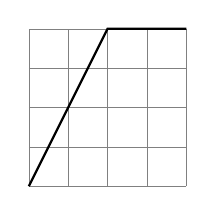
\begin{tikzpicture}
      \draw[step=0.5cm,gray,very thin] (0,0) grid (2,2);
      \draw[thick] (0,0) -- (1,2) -- (2,2);
    \end{tikzpicture}
    \quad
    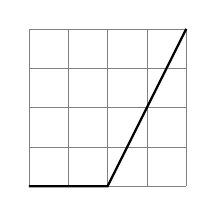
\begin{tikzpicture}
      \draw[step=0.5cm,gray,very thin] (0,0) grid (2,2);
      \draw[thick] (0,0) -- (1,0) -- (2,2);
    \end{tikzpicture}
    \quad
    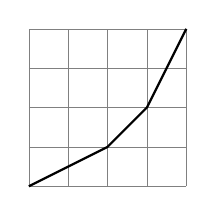
\begin{tikzpicture}
      \draw[step=0.5cm,gray,very thin] (0,0) grid (2,2);
      \draw[thick] (0,0) -- (1,0.5) -- (1.5,1) -- (2,2);
    \end{tikzpicture}
    \caption{Graphs of the functions $\phi_1$, $\phi_2$, and $\phi_3$ respectively.}
    \label{graph-reparametrisation}
  \end{figure}
  
  For (iii) we give a homotopy explicitly. Let us show that $\gamma \star \gamma^\inv \sim_p e_x$. For $t \in [0,1]$, define a path $\gamma_t : [0,1] \to X$ by $\gamma(s) = \gamma(ts)$, and define $G : [0,1] \times [0,1] \to X$ by
  \[
    G(s,t) = (\gamma_t \star \gamma_t^\inv)(s).
  \]
  That $G$ is continuous follows once again from an argument using Remark~\ref{pasting-closed}, and we see that $G$ is a homotopy from $e_x$ to $\gamma \star \gamma^\inv$ since
  \begin{align*}
    G(s,0) &= (\gamma_0 \star \gamma_0^\inv)(s) = \gamma(0) = x = e_x(s),\\
    G(s,1) &= (\gamma_1 \star \gamma_1^\inv)(s) = (\gamma \star \gamma^\inv)(s),\\
    G(0,t) &= \gamma_t(0) = \gamma(0) = x,\\
    G(1,t) &= \gamma_t^\inv(1) = \gamma(0) = x,
  \end{align*}
  for every $s$ and $t$. That $\gamma^\inv \star \gamma \sim_p e_y$ follows by an analogous argument.
\end{proof}


\subsection{The fundamental group}
The idea in this section will be to use the operation $\star$ on path homotopy classes to associate an algebraic structure to any pair $(X,x)$ for $X$ a topological space and $x \in X$. Moreover, when $X$ is path-connected, this structure will form a powerful topological invariant. If $\gamma$ is a path from $x$ to $x$, we say that $\gamma$ is a \word{loop}{{\"o}gla} based at $x$.
\begin{defn}
  Let $X$ be a topological space, and let $x \in X$. Then the \word{fundamental group}{fundamentalgrupp} $\pi_1(X,x)$ is the set of all path homotopy classes of loops based at $x$. 
\end{defn}
\trans{fundamental group}{fundamentalgrupp}
To make sense of the terminology, let us recall a few basic notions from abstract algebra.
\begin{defn}
  A \word{group}{grupp} is a set $G$ with an operation $G \times G \to G$, denoted $(g,h) \mapsto g \cdot h$, an element $e \in G$ called a unit, and a bijection $G \to G$ denoted $x \mapsto x^{-1}$ called the inverse, so that
  \begin{itemize}
    \item $g \cdot (h \cdot k) = (g \cdot h) \cdot k$ for all $g,h,k \in G$,
    \item $e \cdot g = g = g \cdot e$ for all $g \in G$, and
    \item $g \cdot g^{-1} = g^{-1} \cdot g = e$ for all $g \in G$.
  \end{itemize}
  If $G$ and $H$ are groups, then a map $\phi : G \to H$ is called a \word{homomorphism}{homomorfi} if $\phi(g\cdot h) = \phi(g)\cdot\phi(h)$ for all $g,h \in G$. A bijective group homomorphism is called an \word{isomorphism}{isomorfi}.
\end{defn}
\trans{group}{grupp}
\trans{homomorphism}{homomorfi}
\trans{isomorphism}{isomorfi}
\begin{example}
  The integers form a group under the operation $(g,h) \mapsto g+h$. The unit is $0 \in \bbZ$, and if $n \in \bbZ$, then the inverse of $n$ is $-n$.
\end{example}
\begin{example}
  The set $\bbR \setminus \{0\}$ is a group with operation $(g,h) \mapsto gh$. The unit is $1$, and the inverse of $x \in \bbR \setminus \{0\}$ is $1/x$.
\end{example}
\begin{example}
  The set $\GL(n,\bbR)$ of invertible $(n \times n)$-matrices with entries in $\bbR$ is a group under matrix multiplication. The unit is the unit matrix.
\end{example}
\begin{prop}
  The fundamental group $\pi_1(X,x)$ is a group under the operation $\star$ on homotopy classes of loops for any topological space $X$ and any $x \in X$.
\end{prop}
\begin{proof}
  This follows immediately from Theorem~\ref{concatenation-homotopy}.
\end{proof} 

\begin{example}
  \label{fundemental-group-euclidean}
  In Example~\ref{euclidean-path-homotopy} we saw that any two given paths in $\bbR^n$ between the same points were homotopic. This in particular implies that any loop based at a point $x \in \bbR^n$ is null-homotopic; that is, homotopic to $e_x$. In other words,
  \[
    \pi_1(\bbR^n, x) = \{[e_x]\},
  \]
  the trivial group, for all $x \in \bbR^n$.
\end{example}
As the next thing, let us see how $\pi_1(X,x)$ depends on $x$.
\begin{thm}
  Let $X$ be a topological space, and let $\alpha$ be a path from $x$ to $y$ in $X$. Define a map $\hat{\alpha} : \pi_1(X,x) \to \pi_1(X,y)$ by
  \[
    \hat{\alpha}([\gamma]) = [\alpha^\inv] \star [\gamma] \star [\alpha].
  \]
  Then $\hat{\alpha}$ is well-defined and an isomorphism.
\end{thm}
\begin{proof}
  That $\hat{\alpha}$ is well-defined means that $\hat{\alpha}([\gamma]) = \hat{\alpha}([\gamma'])$ whenever $[\gamma] = [\gamma']$, i.e. $\gamma \sim_p \gamma'$. And indeed, if $F: [0,1] \times [0,1] \to X$ is a path-homotopy from $\gamma$ to $\gamma'$, then $G : [0,1] \times [0,1] \to X$, defined by
  \[
    G(s,t) = (\alpha^\inv \star F(\cdot,t) \star \alpha)(s)
  \]
  is a path-homotopy from $\alpha^\inv \star \gamma \star \alpha$ to $\alpha^\inv \star \gamma' \star \alpha$, so $\hat{\alpha}$ is well-defined.

  To see that $\hat{\alpha}$ is an homomorphism, notice that for any $[\gamma], [\gamma'] \in \pi_1(X,x)$, we have
  \begin{align*}
    \hat{\alpha}([\gamma]) \star \hat{\alpha}([\gamma']) &= [\alpha^\inv] \star [\gamma] \star [\alpha] \star [\alpha^\inv] \star [\gamma'] \star [\alpha] \\
      &= [\alpha^\inv] \star ([\gamma] \star [\gamma']) \star [\alpha] = \hat{\alpha}([\gamma] \star [\gamma']).
  \end{align*}
  To see that $\hat{\alpha}$ is a bijection, notice that $\widehat{\alpha^\inv} \circ \hat{\alpha}$ is the identity on $\pi_1(X,x)$ since for any $[\gamma] \in \pi_1(X,x)$, we have
  \[
    (\widehat{\alpha^\inv} \circ \hat{\alpha})[\gamma] = \widehat{\alpha^\inv}([\alpha^\inv] \star [\gamma] \star [\alpha]) = [\alpha] \star [\alpha^\inv] \star [\gamma] \star [\alpha] \star [\alpha^\inv] = [\gamma],
  \]
  and $\hat{\alpha} \circ \widehat{\alpha^\inv}$ is the identity on $\pi_1(X,y)$ by the same reasoning, so $\hat{\alpha}$ is a bijection and thus a group isomorphism.
\end{proof}
\begin{cor}
  If $X$ is a path-connected topological space, then $\pi_1(X,x)$ is independent of $x \in X$ up to isomorphism.
\end{cor}
Because of this result, one often writes $\pi(X) = \pi(X,x)$ for any $x \in X$ when $X$ is path-connected. It is then understood that the equality is really up to isomorphism.
\begin{defn}
  A topological space $X$ is called \word{simply-connected}{enkelt sammanh{\"a}ngande} if it is path-connected and $\pi_1(X)$ consists of a single point.
\end{defn}
\begin{example}
  By Example~\ref{fundemental-group-euclidean}, $\bbR^n$ is simply-connected.
\end{example}

The next result says that for path-connected spaces, $\pi_1$ is a topological invariant. Even when the spaces in question are not path-connected, one obtains a topological invariant by considering the collection groups $\pi_1(X,x_i)$ up to isomorphism, where each of the $x_i$ to a path-component of $X$.

As preparation, suppose that $f : X \to Y$ is a continuous map, and let $x \in X$. Define a map
\[
  f_* : \pi_1(X,x) \to \pi_1(Y,f(x))
\]
by
\[
  f_*([\gamma]) = [f \circ \gamma].
\]

\begin{thm}
  Let $f : X \to Y$ and $g : Y \to Z$ be continuous maps, and let $x \in X$. Then
  \begin{itemize}
    \item[(i)] $f_*: \pi_1(X,x) \to \pi_1(Y,f(x))$ is a well-defined homomorphism,
    \item[(ii)] $(g \circ f)_* = g_* \circ f_*$, and if $\id : X \to X$ is the identity, then so is $\id_* : \pi_1(X,x) \to \pi_1(X,x)$.
    \item[(iii)] Finally, if $f$ is a homeomorphism, then $f_*$ is an isomorphism.
  \end{itemize}
\end{thm}
\begin{proof}
  That $f_*$ is well-defined means that $f \circ \gamma \sim_p f \circ \gamma'$ whenever $\gamma \sim_p \gamma'$. This is the case since if $F$ is a homotopy from $\gamma$ to $\gamma'$, then $f \circ F$ is a homotopy from $f \circ \gamma$ to $f \circ \gamma'$.
  
  To see that $f_*$ is a homomorphism, let $\gamma, \gamma' \in \pi_1(X,x)$. We first notice that by definition of concatenation, we have
  \[
    f \circ ( \gamma \star \gamma') = (f \circ \gamma) \star (f \circ \gamma'),
  \]
  from which it follows that
  \begin{align*}
    f_*([\gamma] \star [\gamma']) &= f_*([\gamma \star \gamma']) = [f \circ (\gamma \star \gamma')] = [(f \circ \gamma) \star (f \circ \gamma')] \\
      &= [ f \circ \gamma] \star [f \circ \gamma'] = f_*([\gamma]) \star f_*([\gamma']),
  \end{align*}
  so $f_*$ is a homomorphism, which shows (i).
  
  Similarly,
  \[
    (g_* \circ f_*)([\gamma]) = g_* ( [f \circ \gamma]) = [g \circ f \circ \gamma] = (g \circ f)_*([\gamma]),
  \]
  which shows the first part of (ii). The last part of (ii) is obvious.
  
  Finally, (iii) follows from (ii) as it follows that $(f^{-1})_*$ satisfies that both $f_* \circ (f^{-1})_*$ and $(f^{-1})_* \circ f_*$ are the identity homomorphisms. Thus $f_*$ is a bijection and therefore an isomorphism.
\end{proof} 

\subsection{Covering spaces and examples}
The main result of this section is a calculation of $\pi_1(S^n)$ for all $n \geq 1$.
\begin{thm}
  We have $\pi_1(S^1) = \bbZ$, and $S^n$ is simply-connected for $n \geq 2$.
\end{thm}
\begin{wrapfigure}{r}{0.3\textwidth}
  \begin{center}
    \begin{overpic}[width=0.28\textwidth]{images/covering}
      \put(37,60){$E$}
      \put(37,13){$B$}
      \put(24,33){$p$}
      \put(18,17){$U$}
      \put(13,91){$p^{-1}(U)$}
    \end{overpic}
  \end{center}
  \caption{A covering map $p : E \to B$.}
  \label{covering-figure}
\end{wrapfigure}
To prove the case $n = 1$, it will be convenient to have at our disposal some basic results about covering spaces.
% \trans{covering space}{?}
% \trans{covering map}{?}
\begin{defn}
  Let $B$ be a topological space. A \wordnotrans{covering space}{?} of $B$ is a topological space $E$ and a continuous surjective map $p : E \to B$, called a \wordnotrans{covering map}{?}, so that each point $b \in B$ has an open neighbourhood $U$ with the property that $p^{-1}(U)$ is a disjoint union of open sets in $E$, each of which is mapped homeomorphically to $U$ by $p$. See Figure~\ref{covering-figure}.
\end{defn}

\begin{example}
  The real line $\bbR$ is a covering space of $S^1$ with covering map $p : \bbR \to S^1$ given by $p(x) = (\cos(2\pi x), \sin(2\pi x))$.
\end{example}

\begin{defn}
  Let $p : E \to B$ be a covering map, and let $f : X \to B$ be a continuous map. A map $\tilde{f} : X \to E$ is called a \word{lifting}{?} of $f$ if $f = p \circ \tilde{f}$.
\end{defn}
\begin{lem}[Path lifting lemma]
  Let $p : E \to B$ be a covering map, let $b \in B$, and let $e \in E$ with $p(e) = b$. Any path $\gamma : [0,1] \to B$ with $\gamma(0) = b$ has a lift $\tilde{\gamma} : [0,1] \to E$ so that $\tilde{\gamma}(0) = e$.
\end{lem}
